\begin{surferIntroPage}{Simple Singularities}{simplesing_A1pm}{Simple Singularities}

 A surface is called \emph{non--singular} or \emph{smooth} if it does
    not have any apex (such points are called singularities). 
    Examples of smooth surfaces are a sphere or a torus (the first 2
    pictures below): 
    \begin{center}
      \vspace{-0.2cm}
      \begin{tabular}{@{}c@{}c@{}c@{\quad}c@{}c@{}c@{}c@{}}
        \begin{tabular}{@{}c@{}}
          smooth:
        \end{tabular}
        &
        \begin{tabular}{@{}c@{}}
          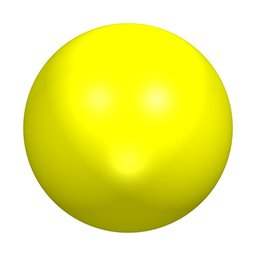
\includegraphics[width=1.1cm]{../../common/images/kugel}
        \end{tabular}
        &
        \begin{tabular}{@{}c@{}}
          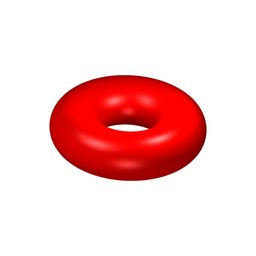
\includegraphics[width=1.1cm]{../../common/images/torus}
        \end{tabular}
        &
        \begin{tabular}{@{}c@{}}
          singular:
        \end{tabular}
        &
        \begin{tabular}{c@{}@{}}
          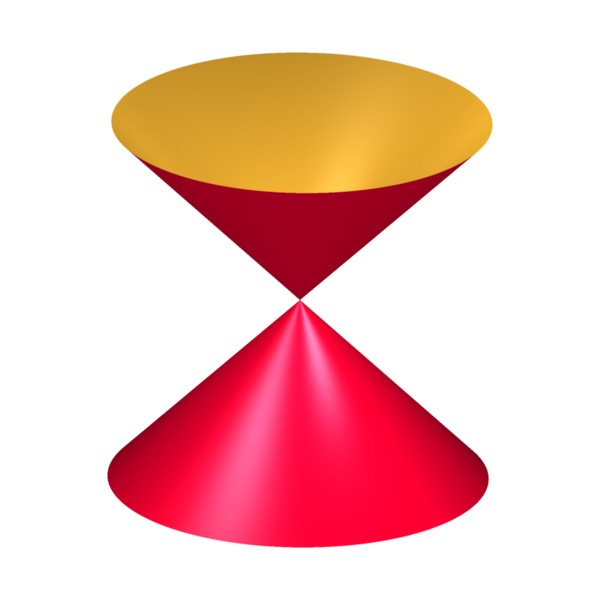
\includegraphics[width=1.1cm]{../../common/images/kegel}
        \end{tabular}
        &
        \begin{tabular}{c@{}@{}}
          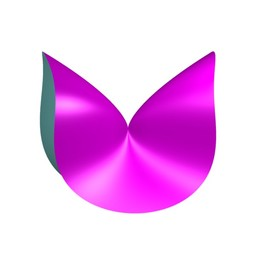
\includegraphics[width=1.1cm]{../../common/images/A2pm}
        \end{tabular}
        &
        \begin{tabular}{c@{}@{}}
          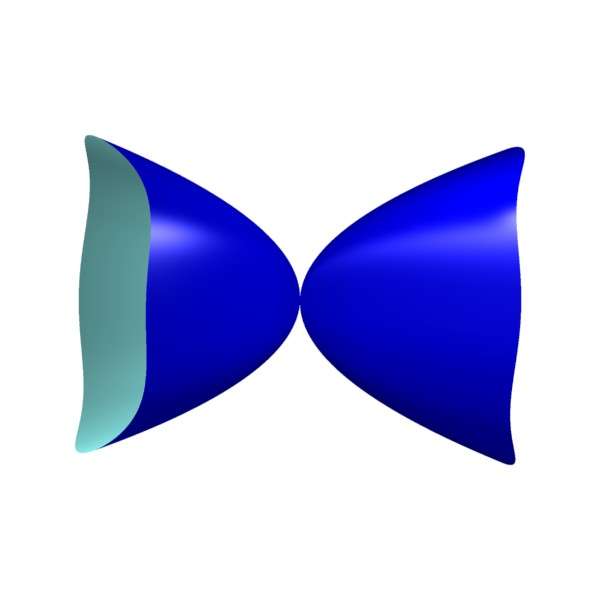
\includegraphics[width=1.1cm]{../../common/images/A3pm_0}
        \end{tabular}
      \end{tabular}
    \end{center}
    \vspace{-0.2cm}
    The so--called \emph{ADE-Singularities} are the simplest singularities.   
    Examples are the singularities of type $A_k^{\pm\pm}$ with equation 
    $x^{k+1}\pm y^2\pm z^2=0$. 
    In the rightmost picture above is an $A_3^{+-}$ singularity (blue), the
    magenta surface is of type $A_2^{+-}$, and the red one of type $A_1^{+-}$
    (called \emph{double cone}).
    The ADE--singularities have amazing relatoins to numerous other branches
    of mathematics, physics, and nature which are still not fully understood. 
    Each $A_k$-singularity can be deformed into $\lfloor\frac{k+1}{2}\rfloor$
    $A_1$-singularities; for an $A_3^{+-}$, we obtain two $A_1^{+-}$s (see
    three pictures on the left):
%    \dontshow{
    % 
    \begin{center}
      \vspace{-0.2cm}
      \begin{tabular}{@{}c@{\quad}c@{}c@{\qquad\quad}c@{\quad}c@{\quad}c@{}}
        \begin{tabular}{@{}c@{}}
          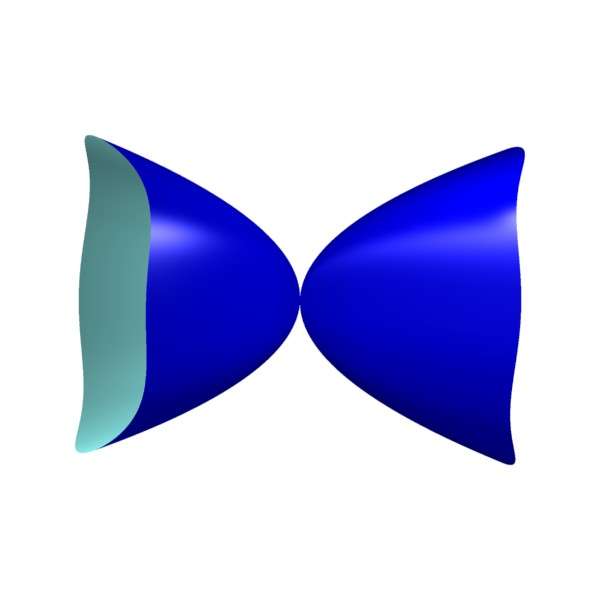
\includegraphics[width=1.2cm]{../../common/images/A3pm_0}
        \end{tabular}
        &
        \begin{tabular}{@{}c@{}}
          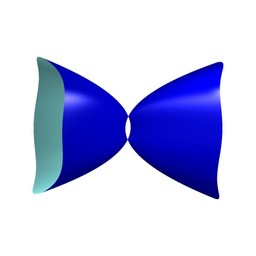
\includegraphics[width=1.2cm]{../../common/images/A3pm_1}
        \end{tabular}
        &
        \begin{tabular}{@{}c@{}}
          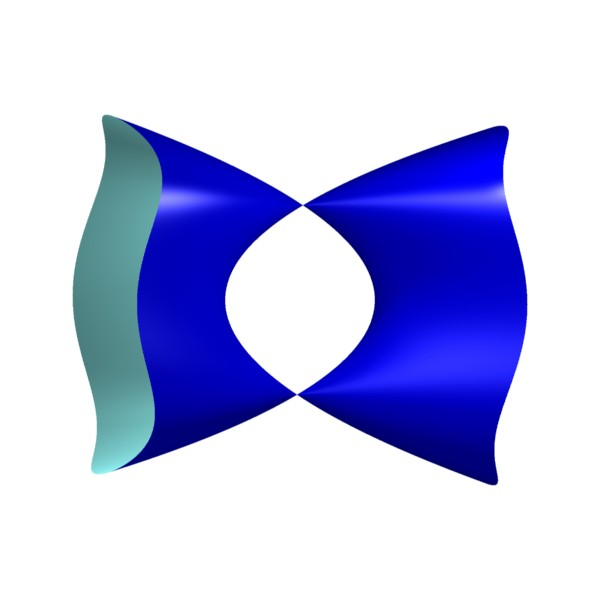
\includegraphics[width=1.2cm]{../../common/images/A3pm_2}
        \end{tabular}
        &
        \begin{tabular}{@{}c@{}}
          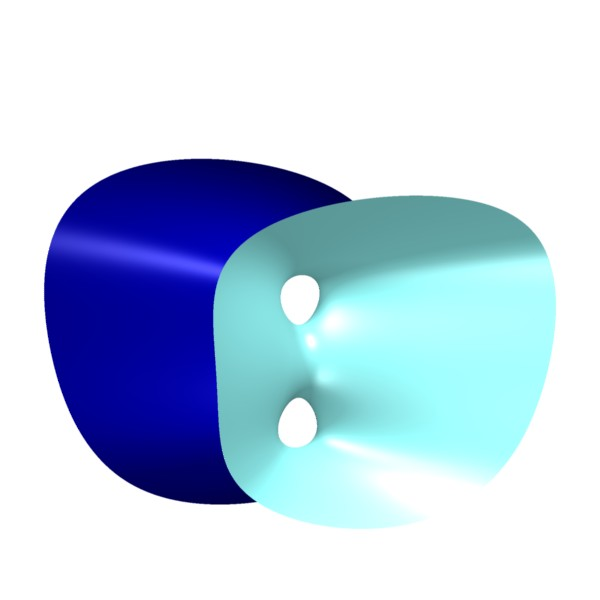
\includegraphics[width=1.2cm]{../../common/images/A3pm_vz_2}
        \end{tabular}
        &
        \begin{tabular}{@{}c@{}}
          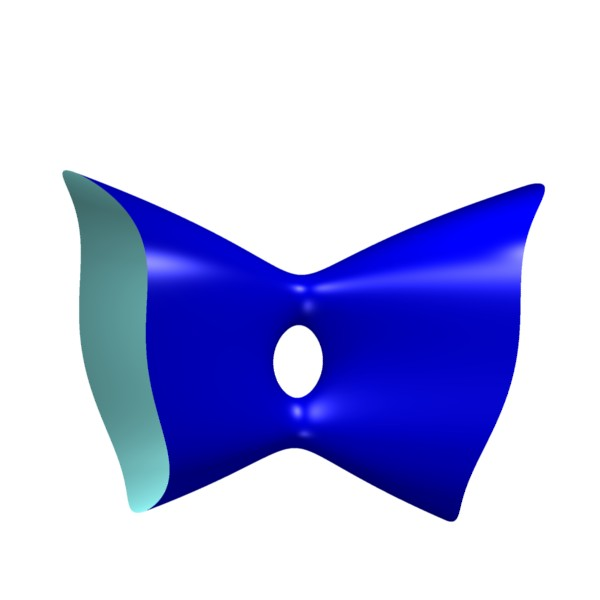
\includegraphics[width=1.2cm]{../../common/images/A3pm_vz_1}
        \end{tabular}
        &
        \begin{tabular}{@{}c@{}}
          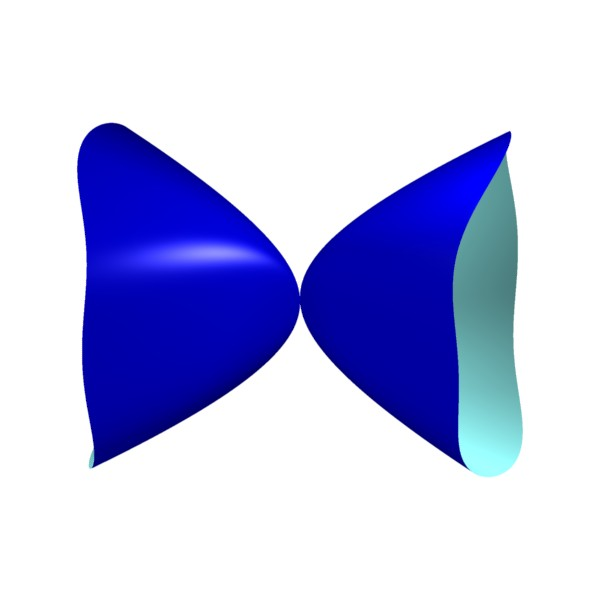
\includegraphics[width=1.2cm]{../../common/images/A3pm_vz_0}
        \end{tabular}
      \end{tabular}
      \\
      \begin{tabular}{@{}c@{\qquad\qquad}c@{}}
          $A_3 \qquad\quad \rightarrow \qquad 2 A_1$
          &
          $2$ Zykel $+$ $1$ Zykel \ $\rightarrow \ A_3$
        \end{tabular}
    \end{center}
%    }
    \vspace*{-0.2cm}
    The index $k$ of the $A_k$--singularities is the so--called \emph{Milnor
      Number} of the singularity; this is the number of \emph{vanishing
      cycles} of the singularity, i.e.\ the number of holes which vanish when
    contracting them to the singular point (see pictures on the right). 

    Gallery created by O.~Labs, www.OliverLabs.net (Saarland Univ.).


\end{surferIntroPage}
